\documentclass[letterpaper]{article}

\usepackage[in,plain]{fullpage}

\usepackage{algorithm}
\usepackage{algorithmic}
\usepackage{amsmath}
\usepackage{amssymb}
\usepackage{graphicx}

\usepackage{subfigure}

\usepackage{color}
\usepackage{hyperref}
\usepackage{url}

\definecolor{col}{rgb}{1.0,0.27,0.0}

\linespread{1.3}

\let\oldthebibliography=\thebibliography
\let\endoldthebibliography=\endthebibliography
\renewenvironment{thebibliography}[1]{%
  \begin{oldthebibliography}{#1}%
    \setlength{\parskip}{0ex}%
    \setlength{\itemsep}{0ex}%
}%
{%
  \end{oldthebibliography}%
}

\begin{document}

\title{\vspace{-50pt} Notes}

\author{}
\date{}

\maketitle

\vspace{-30pt}
\noindent{\bf{\large Preliminaries}}:

Consider the following (linearized) stochastic dynamics and measurement model:
\vspace{-5pt}
\begin{align*}
\bar{\mathbf{x}}_t &= A_t\bar{\mathbf{x}}_{t-1} + B_t\bar{\mathbf{u}}_{t-1} + V_t\mathbf{m}_t, ~~ \mathbf{m}_t \sim \mathcal{N} [\mathbf{0}, M_t]\\
\bar{\mathbf{z}}_t &= H_t\bar{\mathbf{x}}_{t} + W_t\mathbf{n}_t, ~~~~~~~~~~~~~~~~~~~ \mathbf{n}_t \sim \mathcal{N} [\mathbf{0}, N_t].
\end{align*}

We assume that the system is controlled using a linear feedback control policy given by $\bar{\mathbf{u}}_t = L_t\bar{\mathbf{x}}_{t}$. Since the true state deviation, $\bar{\mathbf{x}}_t$, is not available during actual execution, we use a Kalman filter to keep track of a Gaussian estimate of the state deviation, $\hat{\mathbf{x}}_{t}$, during plan execution i.e, $\bar{\mathbf{x}}_t \sim \mathcal{N}[\hat{\mathbf{x}}_t, \hat{\Sigma}_t]$. The revised control policy in terms of the estimate is now given by $\bar{\mathbf{u}}_t = L_t\hat{\mathbf{x}}_{t}$.

The Kalman filter continually performs two steps in an interleaved fashion. A process step first predicts the state deviation and associated variance at the next time-step as:
\begin{align*}
\hat{\mathbf{x}}^{-}_{t} &= A_t \hat{\mathbf{x}}_{t-1} + B_t \bar{\mathbf{u}}_{t-1}\\
\hat{\Sigma}^{-}_{t} &= A_t \hat{\Sigma}_{t-1} A_t^T + V_t M_t V_t^T,
\end{align*}
and a measurement update step that adjusts the prediction and incorporates new information from measurements into the variance as:
\begin{align*}
K_t &= \hat{\Sigma}^{-}_{t} H_t^T (H_t\hat{\Sigma}^{-1}_t H_t^T + W_t N_t W_t^T)^{-1} \\
\hat{\mathbf{x}}_t &= \hat{\mathbf{x}}^{-}_{t} + K_t(\bar{\mathbf{z}}_t - H_t \hat{\mathbf{x}}^{-}_{t}) \\
\hat{\Sigma}_t &= \hat{\Sigma}^{-}_{t} - K_t H_t \hat{\Sigma}^{-}_{t}.
\end{align*}

\noindent{\bf{\large A Priori Belief Propagation}}:

For motion planning under uncertainty, it is important to be able to characterize a priori, the uncertainty in the true state, $\mathbf{x}_t$ (or equivalently, true state deviation $\bar{\mathbf{x}}_t$), of the system. While $\hat{\Sigma}_t$ does represent the uncertainty in the state deviation $\bar{\mathbf{x}}_t$, it also assumes that the mean $\hat{\mathbf{x}}_t$ is available based on measurements obtained during execution. Since the measurements are not available prior to plan execution, it is not possible to determine $\hat{\mathbf{x}}_t$ in advance.

One could incorrectly assume that the obtained measurement would be the same as the nominal state along the plan (maximum likelihood assumption), in which case, $\hat{\mathbf{x}}_t = \mathbf{0}$ and $\hat{\Sigma}_t$ is the uncertainty in the true state. This leads to an underestimation of the true uncertainty from a planning perspective, which can result in computation of unsafe motion plans under uncertainty.

A more principled approach is to consider all possible $\hat{\mathbf{x}}_t$ that could be realized during plan execution. Under the given assumptions, the estimate $\hat{\mathbf{x}}_t$ is normally distributed i.e., $\hat{\mathbf{x}}_t \sim \mathcal{N}[\mu_t, \Gamma_t]$. Using the result from \cite{Bry11} [{\color{red} Note}: I tried deriving this from scratch but had leftover terms in the $\Gamma_t$ derivation that do not go away. I coded it up and this does compute the a priori distributions accurately (Fig. \ref{fig:panel1})], we have:
\begin{align*}
\mu_t &= (A_t + B_t L_{t-1})\mu_{t-1} \equiv \mathbf{0} ~ \forall t \in [0,\ell]\\
\Gamma_t &= (A_t + B_t L_{t-1}) \Gamma_{t-1} (A_t + B_t L_{t-1})^T + K_t H_t \hat{\Sigma}^{-}_{t}.
\end{align*}
The term, $(A_t + B_t L_{t-1})$, is contractive for a stable, closed-loop system i.e., the eigenvalues of the $(A_t + B_t L_{t-1})$ matrix strictly lie within a unit circle for a stable system. The second term, $K_t H_t \hat{\Sigma}^{-}_{t}$, is equivalent to the uncertainty subtracted from the Kalman filter covariance during the measurement update step. Intuitively, the uncertainty subtracted from the variance of the state estimate during execution, is added to the uncertainty of the expected mean of the estimate $\mu_t$.

The state deviation is normally distributed as $\bar{\mathbf{x}}_t \sim \mathcal{N}[\hat{\mathbf{x}}_t, \hat{\Sigma}_t]$, and the state deviation estimate is in turn normally distributed as $\hat{\mathbf{x}}_t \sim \mathcal{N}[\mu_t, \Gamma_t]$. The cumulative distribution of the state deviation is given by the convolution over the two Gaussian distributions as $\bar{\mathbf{x}}_t \sim \mathcal{N}[\hat{\mathbf{x}}_t + \mu_t, \hat{\Sigma}_t + \Gamma_t] \equiv \mathcal{N}[\mathbf{0}, \hat{\Sigma}_t + \Gamma_t]$.

\vspace{10pt}
\noindent{\bf{\large Truncated Belief Propagation}}:

{\color{red} Note:} I tried propagating the variances using equations from the LQG-MP paper, truncating the appropriate sub-matrix $\mathrm{Var}[\bar{\mathbf{x}}_t]$ of the joint variance matrix, $\mathrm{Var}\bigl[\begin{smallmatrix} \bar{\mathbf{x}}_t \\ \hat{\mathbf{x}}_t \end{smallmatrix}\bigr]$, at each time-step and plugging it back in. After a few iterations, the joint covariance matrix would no longer remain positive semi-definite. I found out that this was being caused by the Kalman gains, $K_t$, that were computed based on the original Kalman filter variances $\mathrm{Var}[\hat{\mathbf{x}}_t]$. I then tried truncating the Kalman filter variances but it did not resolve the issue. This is probably incorrect because the truncation does not update the $\mathrm{Cov}[\bar{\mathbf{x}}_t, \hat{\mathbf{x}}_t]$ and $\mathrm{Cov}[\bar{\mathbf{x}}_t, \hat{\mathbf{x}}^{-}_t]$ sub-matrices.

I then tried truncating and propagating the $\hat{\Sigma}_t$ and $\Gamma_t$ matrices separately. The mean, $\mu_t$, is no longer $\mathbf{0}$ i.e., the mean does not lie on the planned path. I use the update equation $\mu_{t+1} = (A_{t+1} + B_{t+1} L_{t})\mu_{t}$ to propagate the mean after truncation and the $\hat{\Sigma}_t$ and $\Gamma_t$ matrices are also propagated as given above. In spite of the fact that this is incorrect because the two Gaussian distributions $\mathcal{N}[\hat{\mathbf{x}}_t, \hat{\Sigma}_t]$ and $\mathcal{N}[\mu_t, \Gamma_t]$ are not centered at the same state and convolving these truncated distributions would yield an incorrect estimate of the actual distribution, this somehow works. I compared the resulting a priori distributions with the maximum likelihood Gaussian distributions computed from the surviving samples at each time-step (out of $100000$ initial samples) and they are a close match. I cannot find any justification for why this should work though. It might be the case that this is a coincidence and works reasonable well for the dynamics/measurement models or the scenarios that have been considered.

\begin{thebibliography}{99.}
\bibitem{Bry11} A. Bry, N. Roy. Rapidly-exploring Random Belief Trees for Motion Planning Under Uncertainty. \emph{IEEE Int. Conf. on Robotics and Automation}, 2011. \url{http://groups.csail.mit.edu/rrg/papers/abry_icra11.pdf}

\end{thebibliography}

\begin{figure}[h]
\begin{center}
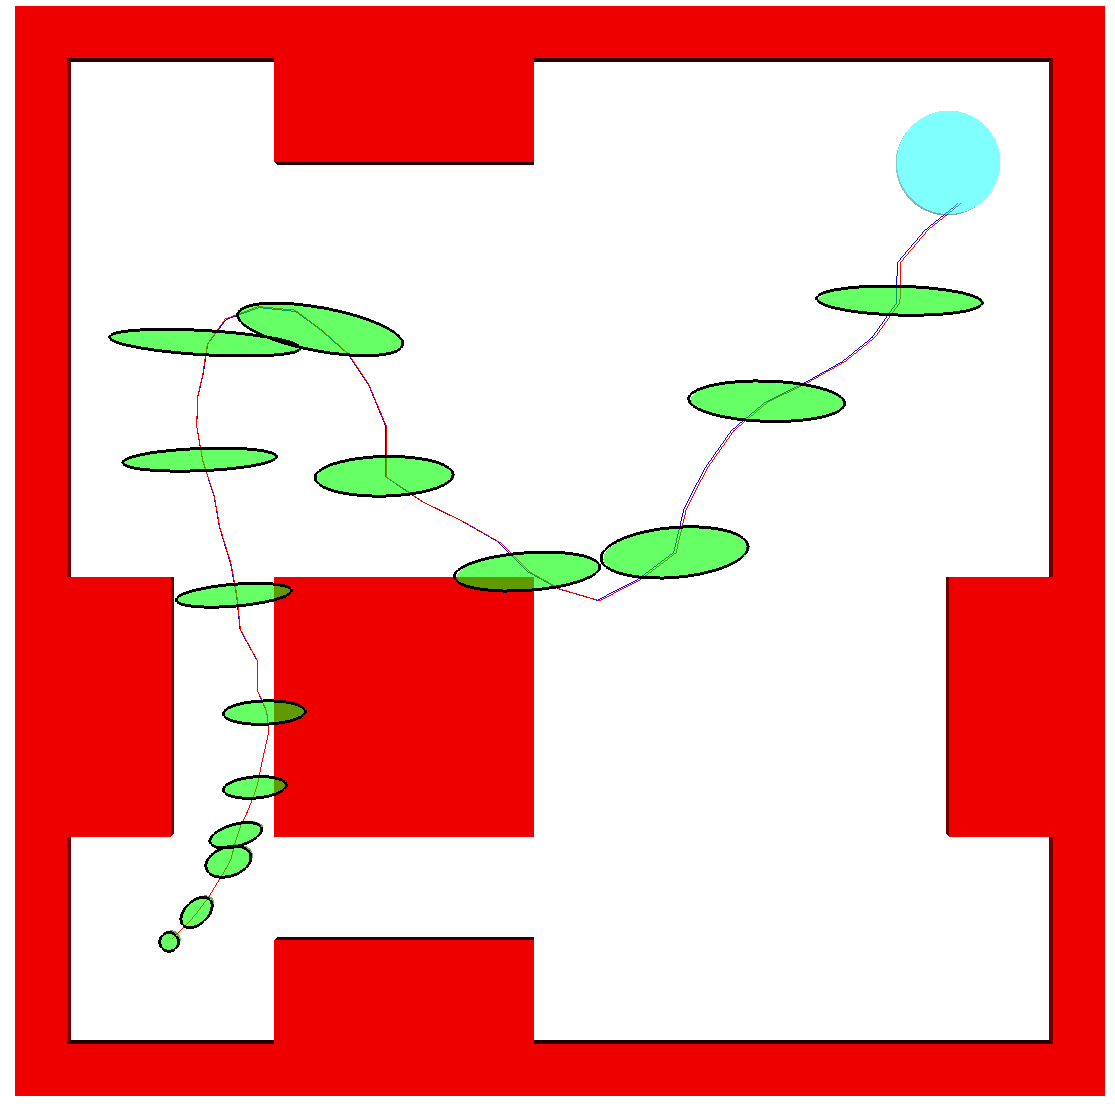
\includegraphics[width=0.49\linewidth]{figures/car-complex1.png}
\vspace{-20pt}
\end{center}
\caption{The a priori distributions computed by \cite{Bry11} (green) exactly matches the maximum likelihood Gaussian distribution computed using $100000$ samples (black). }
\label{fig:panel1}
\end{figure}


\begin{figure}[t]
\begin{center}
\subfigure[\label{fig:car-complex2}]{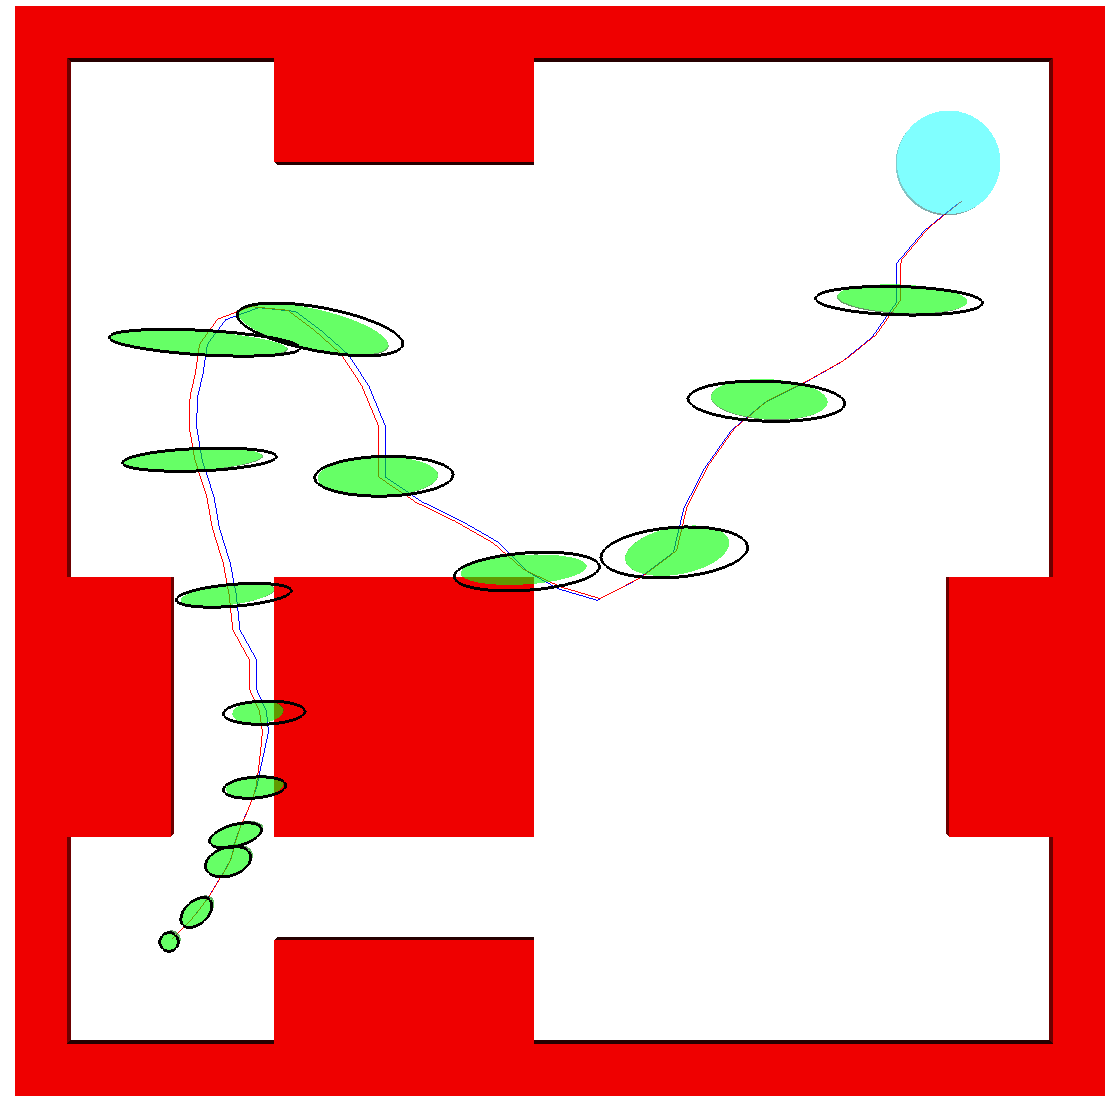
\includegraphics[width=0.49\linewidth]{figures/car-complex2.png}}
\subfigure[\label{fig:car-complex3}]{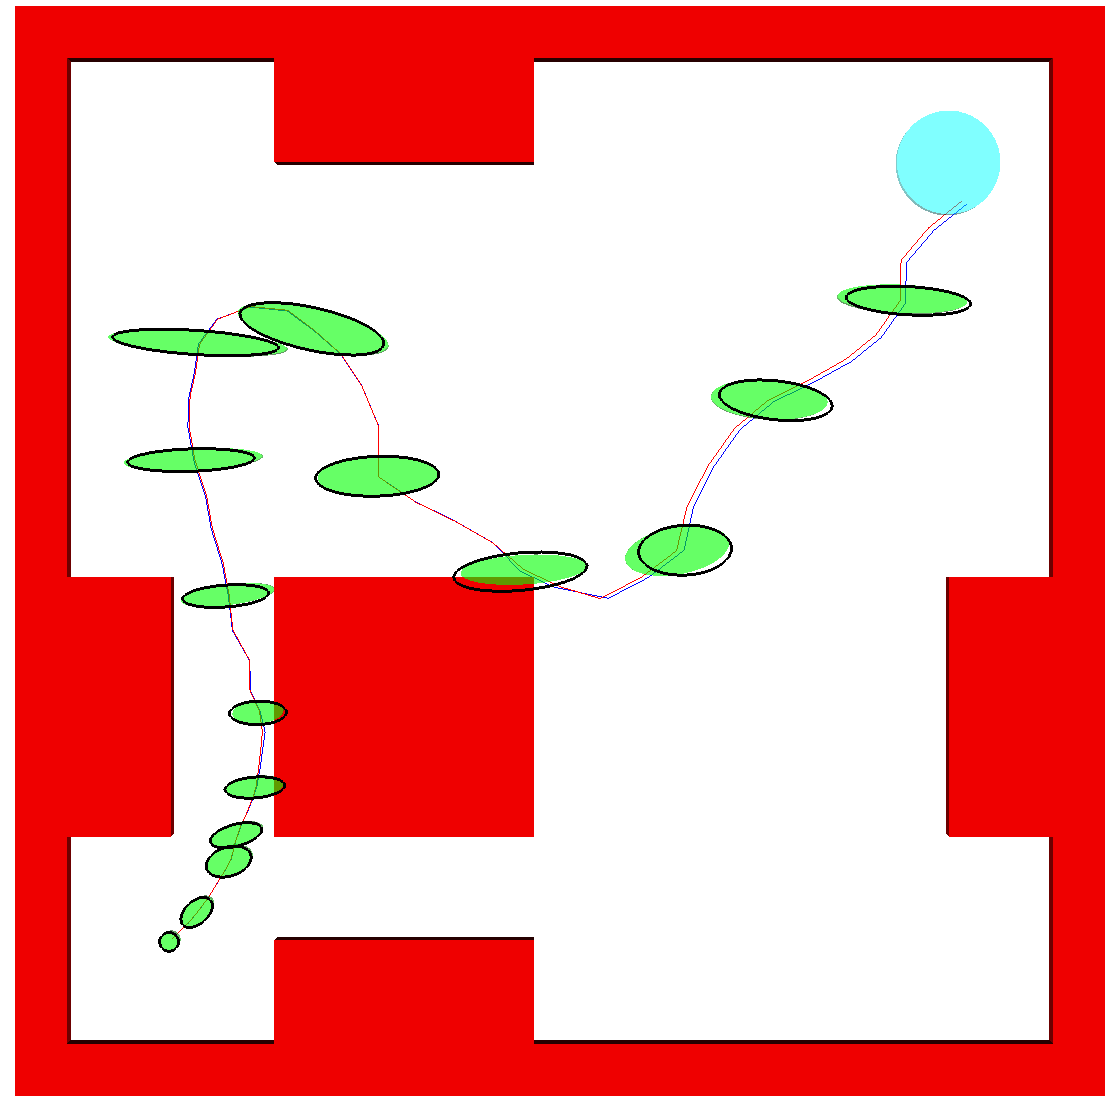
\includegraphics[width=0.49\linewidth]{figures/car-complex3.png}}\\
\vspace{-20pt}
\end{center}
\caption{ (a) The a priori distributions computed by truncating and propagating $\hat{\Sigma}_t$ and $\Gamma_t$ (green) and Gaussian distribution of all samples (black) at each time-step. The red poly-line is the mean path of the truncation method and the blue poly-line is the mean path computed by sampling. (b) The a priori truncated distribution closely matches the Gaussian distribution computed from all surviving samples at each time-step, but the mean paths deviate towards the end, causing the discrepancy.}
\label{fig:panel2}
\end{figure}

\begin{figure}[h]
\begin{center}
\subfigure[\label{fig:car-tube1}]{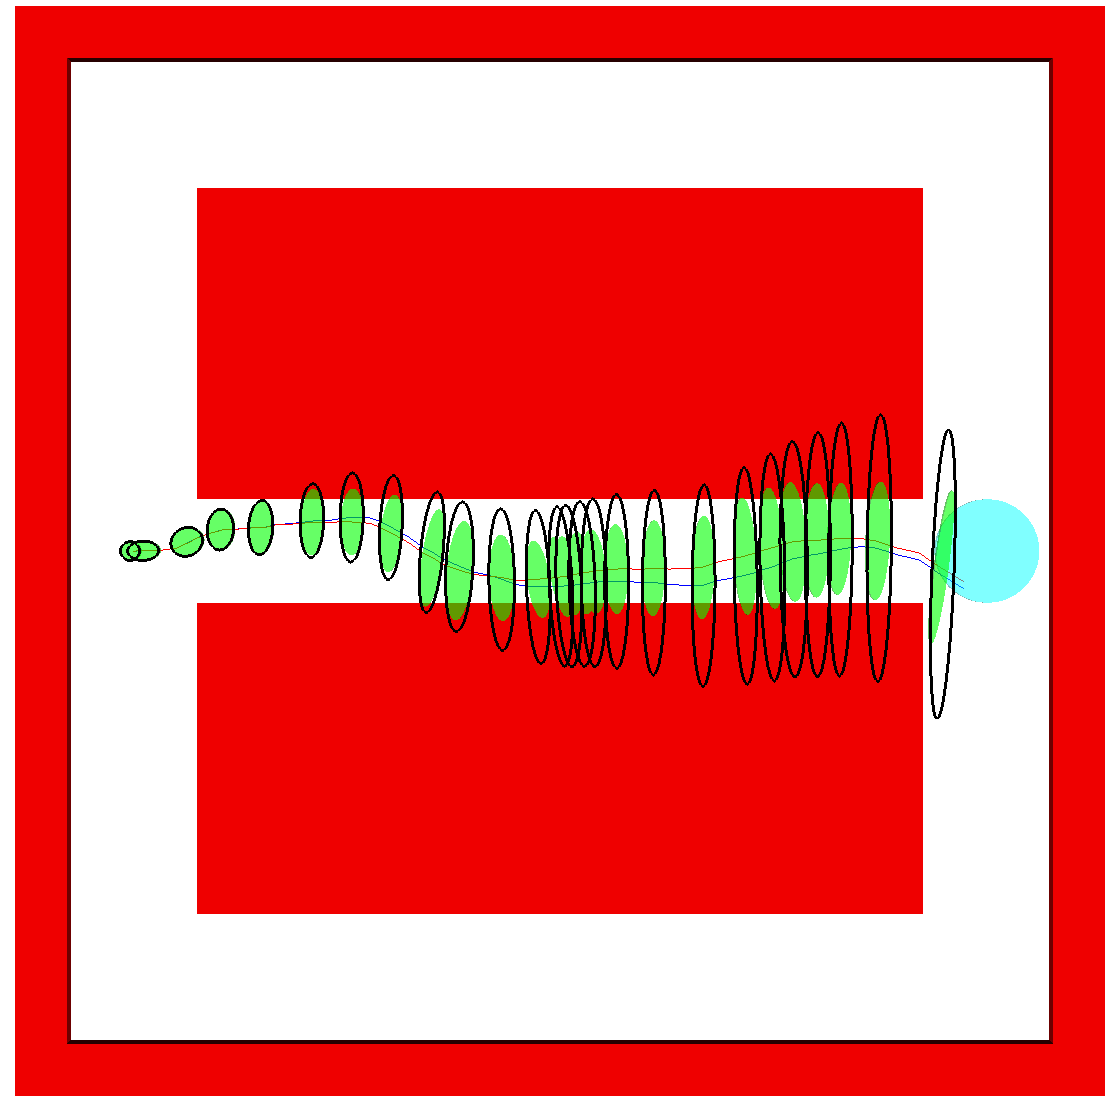
\includegraphics[width=0.49\linewidth]{figures/car-tube1.png}}
\subfigure[\label{fig:car-tube2}]{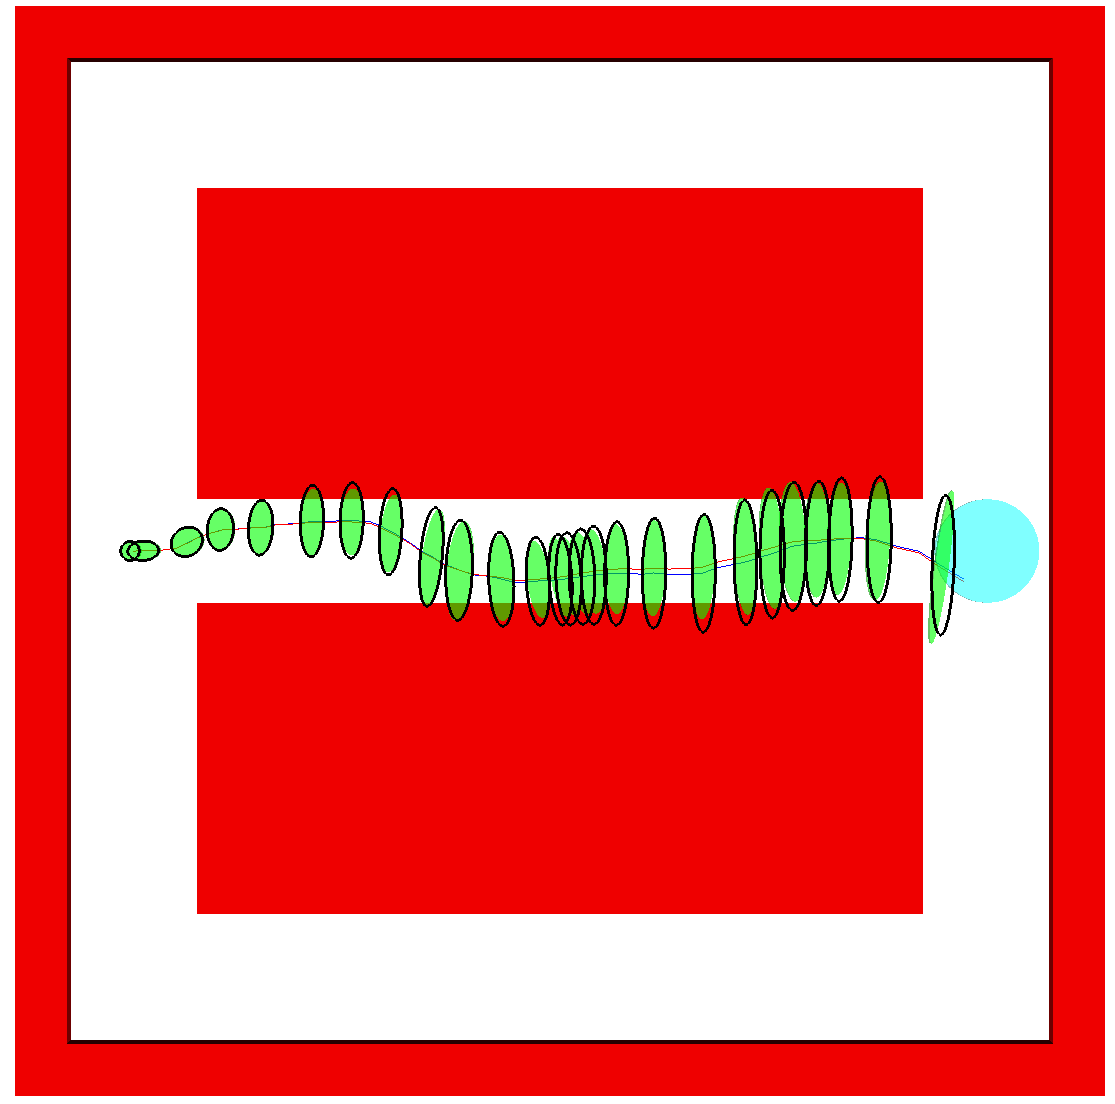
\includegraphics[width=0.49\linewidth]{figures/car-tube2.png}}\\
\vspace{-20pt}
\end{center}
\caption{ Corridor scenario. (a) The a priori truncated distributions (green) and Gaussian distribution of all samples (black) at each time-step. (b) The a priori truncated distribution matches the Gaussian distribution computed from all surviving samples at each time-step.}
\label{fig:panel3}
\end{figure}

\begin{figure}[t]
\begin{center}
\subfigure[\label{fig:car-tube3}]{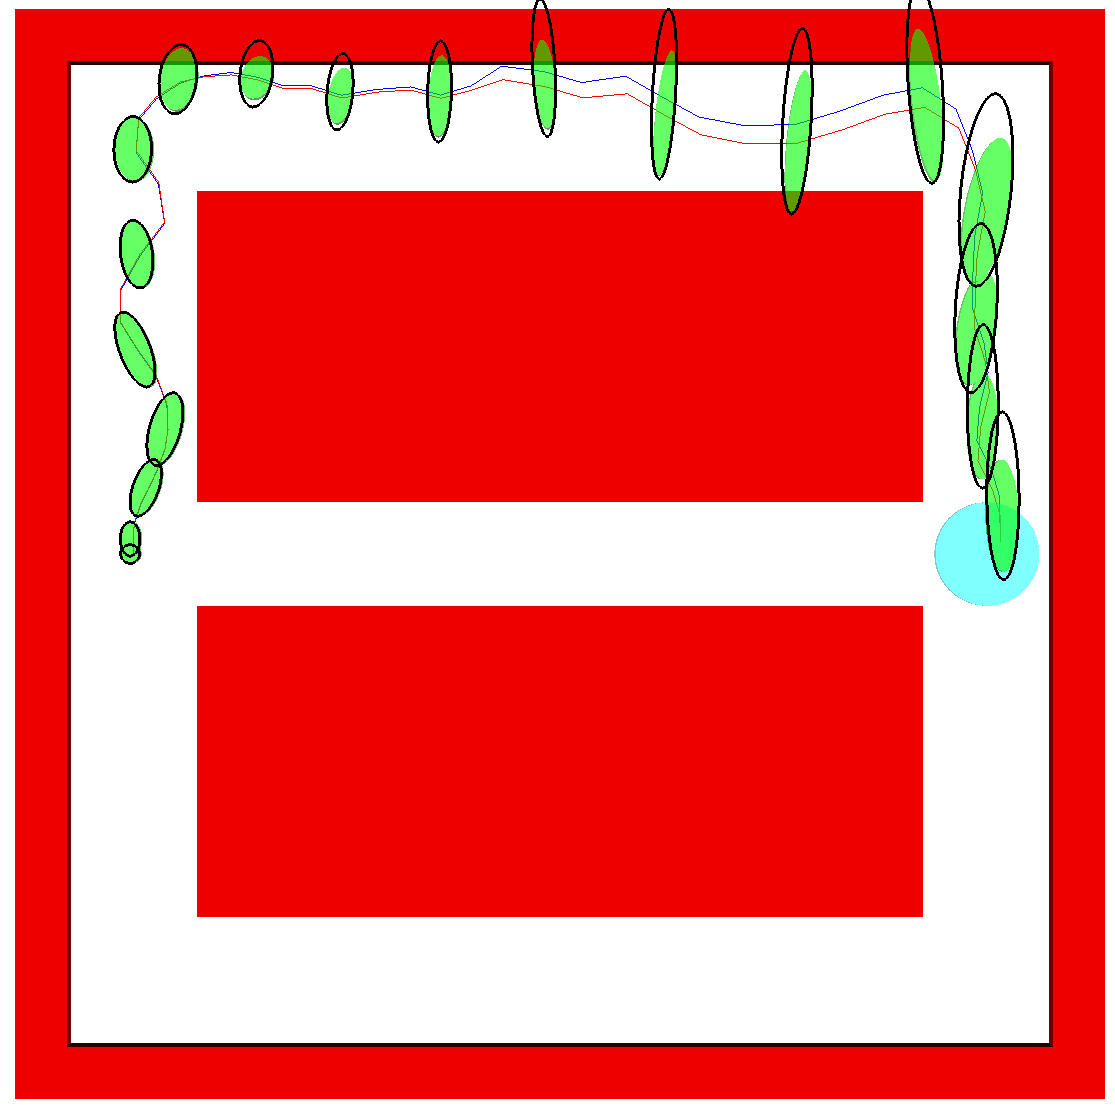
\includegraphics[width=0.49\linewidth]{figures/car-tube3.png}}
\subfigure[\label{fig:car-tube4}]{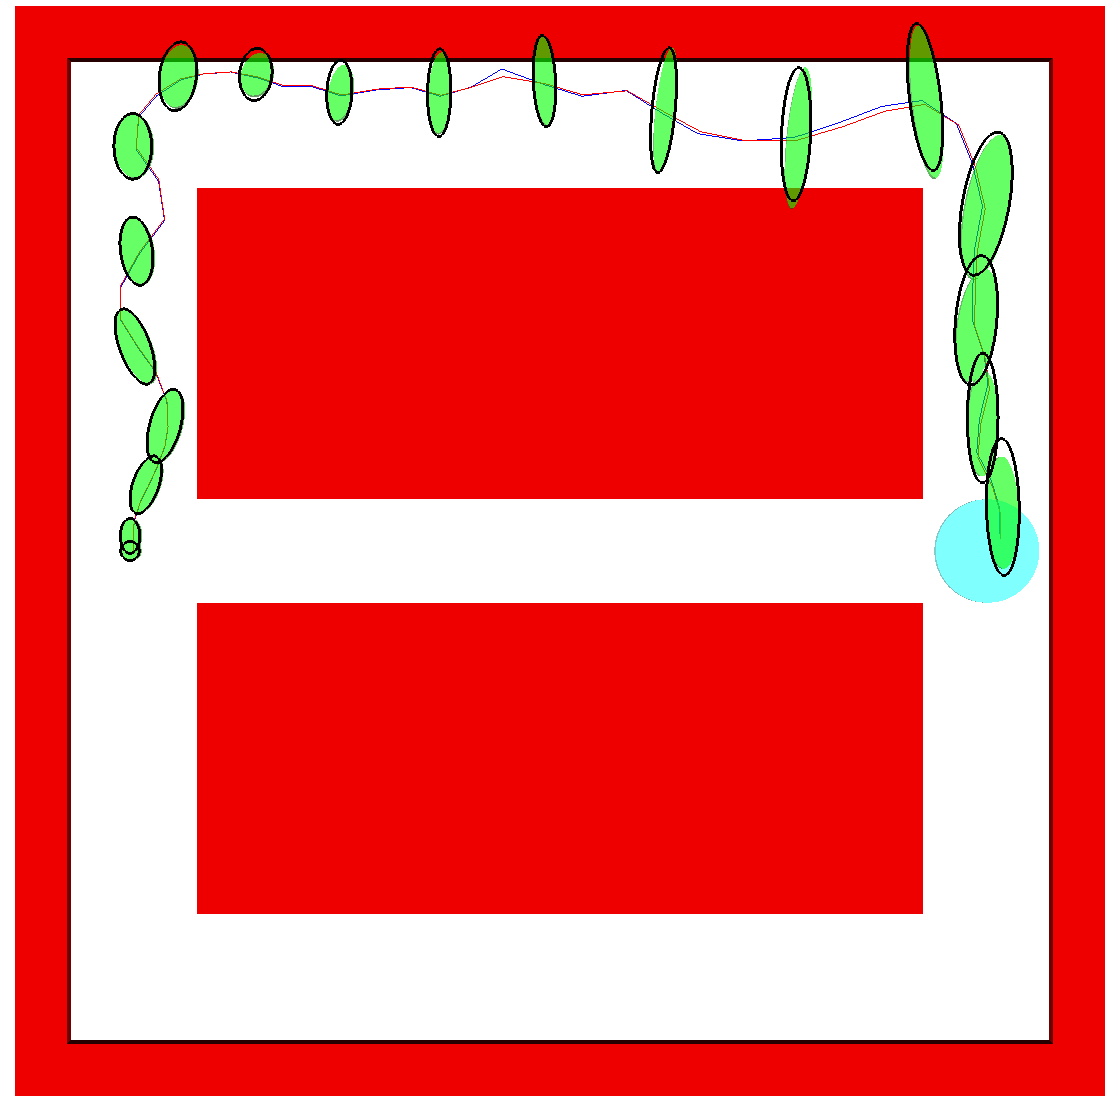
\includegraphics[width=0.49\linewidth]{figures/car-tube4.png}}\\
\vspace{-20pt}
\end{center}
\caption{ Corridor scenario 2: (a) The a priori truncated distributions (green) and Gaussian distribution of all samples (black) at each time-step. (b) The a priori truncated distribution matches the Gaussian distribution computed from all surviving samples at each time-step.}
\label{fig:panel4}
\end{figure}


\end{document} 